\chapter{Global Project Organization}
\label{vl:tc-global}

\section{Global Project Partners}
\label{sec:partners}

The \dword{lbnf} project is responsible for providing both the conventional
facilities and supporting infrastructure (cryostats and cryogenic
systems) which house the \dword{dune} far detector modules. \dword{lbnf} is a
U.S. \dword{doe} project incorporating in-kind contributions from
international partners and is headed by the \dword{lbnf} Project Director who
also serves as the \fnal Deputy Director for \dword{lbnf}.  The \dword{dune}
project is responsible for providing all components required for
fabricating the detector modules. \dword{dune} is an international project
with some \dword{doe} contributions that is directed by \dword{dune}
collaboration management. The organization of the global project 
is shown in Figure~\ref{fig:DUNE_global}.
\begin{dunefigure}[Global project organization]{fig:DUNE_global}
  {Overall global  \dword{lbnf}/\dword{dune} organization.}
  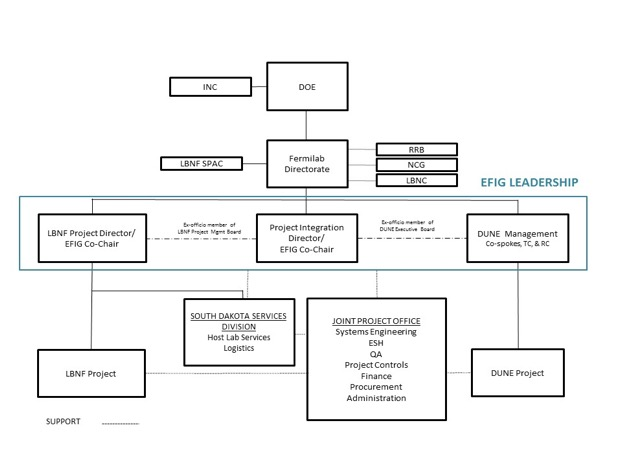
\includegraphics[width=0.99\textwidth]{DUNE_global}
\end{dunefigure}

In addition to the \dword{lbnf} and \dword{dune} pieces, the overall
integration and installation of the detector modules and supporting
\dword{lbnf} infrastructure in the underground areas at \surf
post-excavation are defined as separate project elements.  These
elements fall under the responsibility of the \dword{ipd}, who is
appointed by and reports directly to the \fnal director.  To ensure
the best possible coordination across all elements of the global
project, the \dword{ipd} connects to the facilities and detector
construction projects, respectively, through ex-officio positions on
the \dword{lbnf} Project Management Board and \dword{dune}
\dword{exb}.

In addition to taking responsibility for the integration and
installation of the detectors and supporting \dword{lbnf}
infrastructure in the underground caverns post-excavation, the
\dword{ipd} works closely with the \dword{lbnf} and \dword{dune}
project teams in advance of these activities to coordinate planning
and assure the proper integration of detector elements within the
supporting infrastructure.  \dword{dune} collaboration management
takes direct responsibility for design and construction of the far
detector elements and supports detector integration and installation
activities by providing dedicated personnel and equipment resources.
\dword{lbnf} project management is responsible for construction of the
conventional detector facilities (up to the point of beneficial
occupancy) as well as the design and construction of the supporting
detector infrastructure (cryostats and cryogenic systems). \dword{lbnf} also
has dedicated resources to support the integration and installation of
this infrastructure, although the overall coordination of the
associated activities in the underground area falls under the
responsibility of the \dword{ipd}.

\section{\dword{efig}}
\label{sec:efig}

The \dword{efig} is the body responsible for the required high-level
coordination between the \dword{lbnf} and \dword{dune} projects.  The
\dword{efig} is co-chaired by the \dword{lbnf} Project Director and
the \dword{ipd}. \dword{efig} leadership also incorporates the four
members of the \dword{dune} collaboration management team
(co-spokespersons, \dword{tcoord}, and \dword{rcoord}).  The
\dword{efig} is responsible for steering the global project and
operates via the consensus of its leadership team.  If an issue arises
for which consensus cannot be achieved, responsibility for resolving
the issue is passed to the \fnal Director.

\section{\dword{jpo}}
\label{sec:jpo}

The \dword{efig} is augmented by a \dword{jpo} that supports the
\dword{lbnf} and \dword{dune} projects as well as the integration
effort across \dword{lbnf} and \dword{dune}. The \dword{jpo} combines
project activities and functions that exist within the \dword{lbnf} and \dword{dune}
projects to ensure that they are properly coordinated across the
entire enterprise.  Members of the \dword{jpo} organization are drawn directly
from the project teams supporting \dword{lbnf} and \dword{dune} as well as the team
supporting the overall integration effort.  Figure~\ref{fig:DUNE_jpo} shows the
current organizational structure of the \dword{jpo}, indicating the members
being pulled in from the \dword{lbnf} (LBNF), \dword{dune} (TC) and \dword{lbnf}/\dword{dune}
Integration (NP) project teams.
\begin{dunefigure}[\dword{jpo} org chart]{fig:DUNE_jpo}
  {\dword{jpo} organization.}
  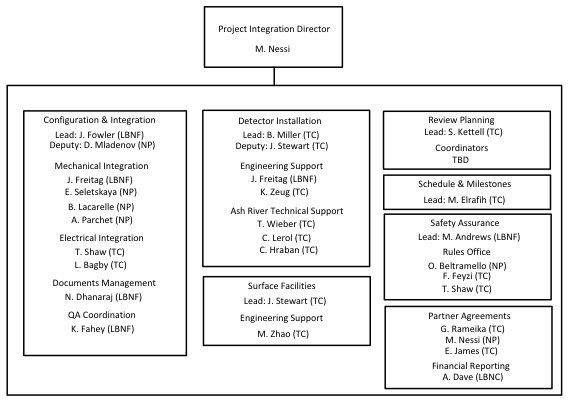
\includegraphics[width=0.99\textwidth]{DUNE_jpo}
\end{dunefigure}
The team members focusing on specific project activities and functions
within the \dword{jpo} are typically those carrying equivalent
responsibilities within their home organization.  For example, the
\dword{jpo} team responsible for building the fully integrated model
of the detector within its supporting infrastructure and the
surrounding facility includes the members of the \dword{lbnf} and
\dword{dune} project teams responsible for integrating the individual
elements.

\section{Coordinated Global Project Functions}
\label{sec:global_project}

\dword{jpo} functions include global project configuration and integration,
installation planning and coordination, scheduling, safety assurance,
technical review planning and oversight, development of partner
agreements and financial reporting.  At the time when the \dword{lbnf}
Conventional Facilities subproject delivers beneficial occupancy of
the underground detector caverns at \surf, the \dword{jpo} will evolve into a
stand-alone organization that takes responsibility for the onsite
activities at \surf required to install the detectors and supporting
infrastructure under the direction of the \dword{ipd}.
Some members of the current \dword{lbnf} and \dword{dune} project teams are
expected to become fully embedded within the \dword{jpo} at that point in
time.  The full \dword{jpo} organization required to assume responsibility for
post-excavation activities at \surf is described in Chapter~\ref{ch:tc-jpo}.
JPO functions associated with its global project coordination role
are described in the following sections.

\subsection{Safety}
\label{sec:dune_safety}

To ensure a consistent approach to safety across the global project,
there is a single Project \dword{esh} manager who reports directly to
the \dword{lbnf} Project Director, \dword{ipd} and \dword{dune}
Management (via the \dword{dune} \dword{tcoord}).  This individual
directs separate safety teams responsible for implementing the global
project \dword{esh} program within both the \dword{lbnf} and
\dword{dune} projects as well as the \dword{lbnf}/\dword{dune}
integration and installation activities at \surf.  The Project
\dword{esh} manager works directly with the \fnal and \surf safety
teams to ensure that all project-related activities comply with the
rules and regulations of the host organizations.  For example, the
Project \dword{esh} manger works directly with the host safety
organizations to develop the rules and regulations governing work in
the underground areas at \surf, which are then consistently applied
across all underground project activities.

The \dword{jpo} includes an engineering safety assurance team that
defines a common set of design and construction rules (mechanical and
electrical) to ensure consistent application of engineering standards
and engineering documentation requirements across the global project.
This team also works with the Project \dword{esh} manager to develop
equivalencies in codes and standards across the international project
as needed.  Following on lessons-learned from the processes employed
for the \dword{protodune} detectors, an important mandate of the
engineering safety assurance team is to ensure that safety issues
related to component handling and installation are incorporated within
the earliest stages of the design review process.  The \dword{jpo}
team will incorporate engineering resources to perform independent
validation of required mechanical analyses that ensure the structural
integrity of detector components through all stages of construction,
installation, and operation.

\subsection{Engineering Integration}
\label{sec:dune_engineering}


A central \dword{jpo} engineering team is responsible for building an
integrated model of the detectors within their supporting
infrastructure and the conventional facilities that house them.  The
team builds and maintains a full 3D CAD model of everything in the
underground detector caverns from the models of the individual
components provided by the \dword{lbnf} and \dword{dune} design teams.
Starting from the latest, approved version of the full CAD model, the
\dword{jpo} team incorporates approved changes as they are received
and runs a series of checks to ensure that no errors or spatial
conflicts are introduced into the model.  As part of this process a
series of 2D control drawings are produced from the 3D CAD model to
validate adherence with a selection of critical component-to-component
clearances that exist within the integrated model.  The updated
working model is also passed back to the individual \dword{lbnf} and
\dword{dune} design teams to validate that the introduced
modifications match with expectations.  After receiving the
appropriate sign-offs from all parties, the \dword{jpo} team tags a
new frozen release of the model and makes it available to the design
teams as the current release against which the next set of design
changes will be generated.

Electrical engineers are also incorporated within the central
\dword{jpo} team to ensure proper integration and installation of the
detector electrical components.  This team is responsible for ensuring
that detector grounding and shielding requirements, the maintenance of
which are critical for detector performance, are strictly adhered to.
The team oversees the layout of electronics racks and cable trays both
on the top of the cryostats and within the \dword{cuc} counting room
that hosts the DAQ electronics.  It also oversees the design of the
power and cooling distribution systems that are required to support
the electronics infrastructure.

The \dword{jpo} engineering team is responsible for documenting and
controlling the interfaces between the \dword{lbnf} and \dword{dune} projects as well
as the interfaces between these projects and the \dword{lbnf}/\dword{dune} integration
and installation activities at \surf.  To define these interfaces, the
\dword{jpo} team develops formal documents, which subsequent to the approval
of the relevant managers are placed under signature and versioning
control.  These documents are monitored regularly to ensure that no
missing scope or technical incompatibilities are introduces at the
boundaries between the projects.


\subsection{Change Control and Document Management}
\label{sec:dune_changecontrol}

The global project partners have agreed to adopt the formal change
control process developed previously for the \dword{lbnf} project.
The change control process applies to proposed modifications of
requirements, technical designs, schedule, overall project scope and
assigned responsibilities for individual scope items.  The formal
global change control process is described in \dword{dune} DocDB-82.
The process includes separate decision paths for items affecting only
\dword{dune} or \dword{lbnf} and incorporates an additional pathway
for items affecting both projects.  A hierarchy of decision-making
layers are built into each pathway based on pre-determined thresholds
related to the extent of the proposed change.  The lowest-level change
control body for modifications affecting both \dword{lbnf} and
\dword{dune} is the \dword{efig}.  The \dword{jpo} team includes a
Configuration Manager who is responsible for formally implementing
changes that are approved through this process.  After technical
changes are incorporated into the global 3D CAD models, the lead
\dword{lbnf}/\dword{dune} systems engineer is responsible for checking production
drawings and verifying that no potential space conflicts have been
introduced.  Under the direction of the Configuration Manager, all
project changes are documented in detail and signed-off on by the
appropriate project partners using the \dword{lbnf} change control tool.

The Configuration Manager will also be responsible for administrating
and managing the global project document management system, which will
be hosted in EDMS.  All technical documents and drawings will be
stored in the \dword{edms} system under formal signature and
versioning control.  A Product Breakdown Structure (PBS) database will
be maintained to track the history of each detector (and supporting
infrastructure) component through construction, assembly, testing,
transport and installation.  The global project \dword{qa} manager who
sits within the \dword{jpo} has responsibility for ensuring that all
necessary documents and testing results used to validate component
quality are uploaded into the PBS database.

\subsection{Schedule and Milestones}
\label{sec:dune_schedule}

The \dword{jpo} team is responsible for creating a single global
project schedule incorporating all \dword{lbnf} and \dword{dune}
project activities in addition to the \dword{lbnf}/\dword{dune}
integration and installation activities at SURF with their correct
interdependencies in order to track the overall progress of the global
project.  The project partners have agreed that the global schedule
will be maintained within the same P6 framework used to plan and
status the resource-loaded schedule of activities associated with the
U.S. contributions to \dword{lbnf} and \dword{dune}.  Activities that
fall under the responsibility of other international partners are
included and directly linked within the P6 schedule but do not
incorporate the associated resource information required for
U.S. activities.  The non-U.S. activities are not tracked using the
formal EVMS procedures required for U.S. project activities but rather
just through regular assessments of their progress towards completion
by the management teams responsible for those activities.  A
substantial number of milestones are embedded into the schedule at a
level of granularity that ensures high-level tracking of project
progress towards completion.

\subsection{Review Process}
\label{sec:dune_review}

To achieve coherency in the review process across the global
enterprise, reviews will be coordinated through the \dword{jpo}.
Direct responsibility for design and production reviews lies with the
\dword{lbnf} project management team and \dword{dune} collaboration
management for infrastructure and detector components, respectively,
while the \dword{ipd} has the lead responsibility for installation and
operational readiness reviews.  Central coordination through the
\dword{jpo} ensures that issues related to installation and operation
are incorporated within all stages of the review process.  Safety
issues related to the handling and installation of components are
addressed starting from the earliest design reviews through the
development of detailed engineering notes containing the required
structural analysis.  The \dword{jpo} team is also responsible for
tracking review recommendations and closing them as appropriate based
on the resulting actions.

\subsection{Partner Agreements and Financial Reporting}
\label{sec:dune_agreements}

Partner contributions to all project elements will be detailed in a
series of written agreements.  In the case of \dword{lbnf}, these
contributions will be spelled out in bilateral agreements between
\dword{doe} and each of the contributing partners.  In the case of
\dword{dune}, there will be a single Memorandum of Understanding (MOU)
detailing the contributions of all participating partners.  The MOU
will detail the deliverables being provided by each partner and
summarize required contributions to common items, for which the
collaboration assumes shared responsibility.  A series of more
technical agreements describing the exact boundaries between partner
contributions and the terms and conditions under which they will be
delivered will lie just beneath the primary agreements.  The
\dword{jpo} will coordinate production of these agreements and work to
obtain the appropriate partner sign-offs on each.  The financial
reporting required for partners to track common fund contributions
will also be organized through the \dword{jpo}.

\section{ProtoDUNE Experience}
\label{sec:dune_protodune}

The structure of the global project is based heavily on the
organization that successfully executed the construction,
installation, commissioning and operation of the \dword{protodune}
detectors at CERN.  The on-site team at CERN responsible for the
overall integration and installation of detector and infrastructure
components within the test beam facility played a critical role in the
successful execution of the \dword{protodune} program.  The separate
projects responsible for the construction of the detector and
infrastructure components interacted effectively with the central,
onsite team to minimize the number of issues encountered during the
installation and commissioning process.  In cases where issues did
arise, the project teams were able to work effectively with their
counterparts on the onsite team to reach a quick resolution.

Some lessons-learned from the \dword{protodune} experience have been
applied in creating the global project organization for the DUNE Far
Detectors.  The integration of installation safety issues into the
early stages of the design review process is one such example.  Delays
were encountered in getting approvals for the installation of some
\dword{protodune} detector components stemming from the absence of a
coordinated approach in the review process for these items.  The
creation of a \dword{jpo} team with responsibility for organizing a
coherent review process addresses this issue directly.  In general,
the successful implementation of the \dword{protodune} detectors
demonstrates the capacity of the organizational structure to safely
execute the project and meet performance requirements.
